\textbf{COLUNI 2026 -- Questão 34}\par\medskip Um estudante brasileiro residente em Porto Alegre (RS) decidiu participar de uma competição internacional \textit{online} organizada por uma universidade em São Francisco, nos Estados Unidos da América. A organização informou que a prova começará pontualmente às 15h, horário local de São Francisco.

\begin{figure}[htbp]
\centering
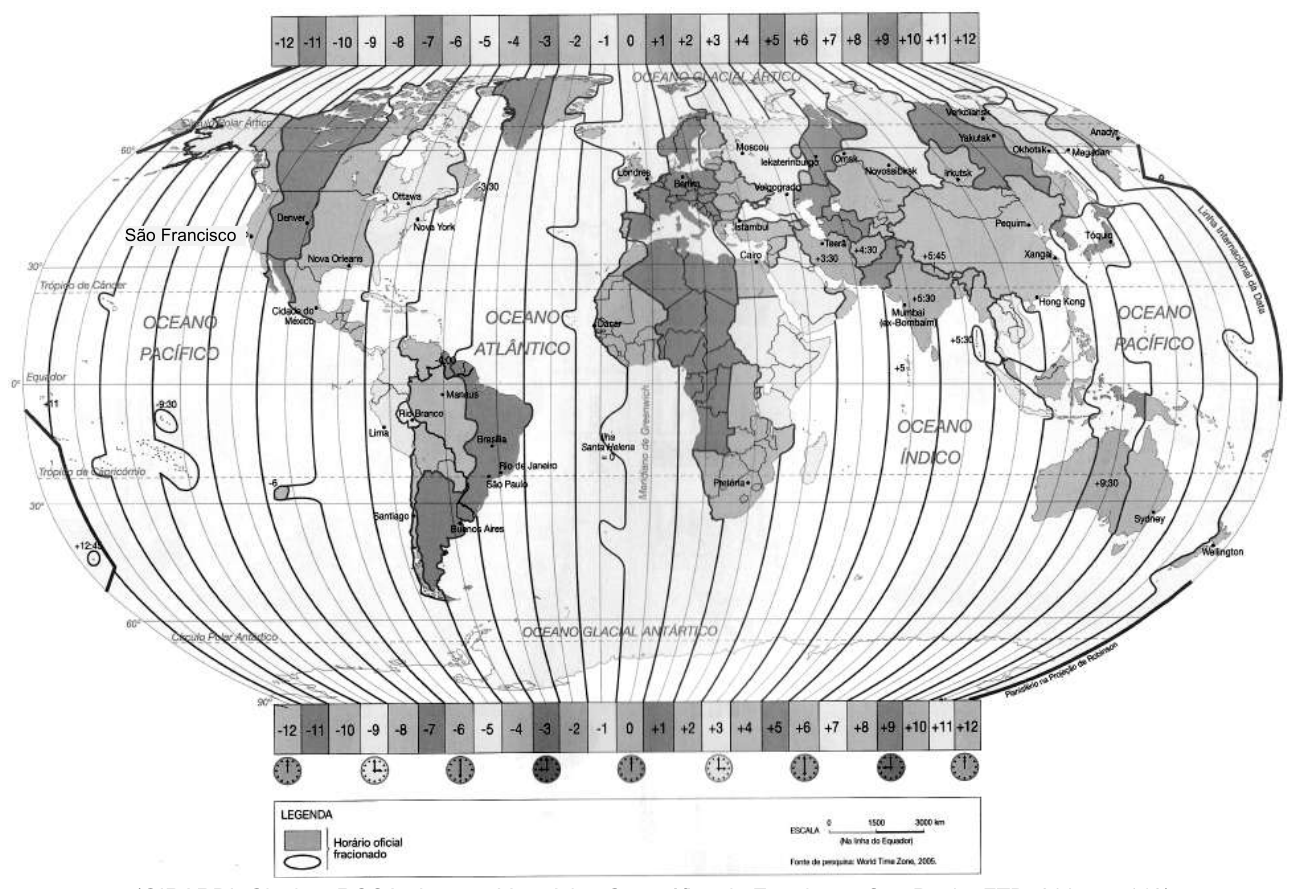
\includegraphics[width=0.92\linewidth]{static/simulados/coluni/figuras/2026/questao-34/figura-1.png}
\end{figure}

(GIRARDI, Gisele e ROSA, Jussara Vaz. Atlas Geográfico do Estudante. São Paulo: FTD, 2005, p. 142)

Considerando os conhecimentos geográficos, as informações fornecidas e a hora local em Porto Alegre, o estudante deverá estar \textit{online} para a prova às:\begin{enumerate}
\item 15h, pois as duas cidades se localizam no mesmo fuso horário.
\item 20h, pois o horário de Porto Alegre (RS) é 5 horas adiantado em relação a São Francisco (EUA).
\item 10h, pois o horário de São Francisco (EUA) é 5 horas adiantado em relação a Porto Alegre (RS).
\item 21h, pois as duas cidades se localizam em hemisférios distintos.\end{enumerate}